
%%%%%%%%%%%%%%%%%%%%%%%%%%%%%%%%%%%%%%%%%%%%%%%%%%%%%%%%
% LaTex Template for proposals within the              %
% DFG Research Unit Program                            %         
%Planet Formation Witnesses and Probes: Transition disks
% August 2016                                            %                           
%                                                      %
%%%%%%%%%%%%%%%%%%%%%%%%%%%%%%%%%%%%%%%%%%%%%%%%%%%%%%%%
%
% 
%
% This template may be used to prepare proposals in latex.
%
%
% The project description, including publication list, should be no more than 20 pages
% in length. It should be self-explanatory and not require reviewers to read the 
% literature that is quoted or enclosed.

\documentclass[10pt,fleqn,twoside]{article}

%%%%%%%%%%%%%%%%% GET THE STYLE STUFF %%%%%%%%%%%%%%%%%%%

%%%% USE ARIAL FONT %%%%%%%%%%%%%%%%%%%%%%%%%%%%%%%%%%%%%%%%%%%%%%%%%%%%%%
\usepackage{helvet}
\renewcommand\familydefault{phv}

%%%% INCLUDE NECESSARY PACKAGES %%%%%%%%%%%%%%%%%%%%%%%%%%%%%%%%%%%%%%%%%%
%\usepackage{babel}
\usepackage[UKenglish]{babel}
\usepackage{amsmath}
\usepackage{amssymb}
\usepackage{fancyhdr}
\usepackage{natbib}
\usepackage{ae,aecompl}
\usepackage{graphicx}
\usepackage{palatino}
\usepackage[T1]{fontenc}
\usepackage[right]{eurosym}
\usepackage{rotating}
\usepackage{epsf}
\usepackage{setspace}
\usepackage{xspace}
\usepackage{multicol}
\usepackage{siunitx}
%\usepackage{caption}

\usepackage{sfmath}

\usepackage[utf8]{inputenc}

% ========= hyperref & Colors & Links ===========
\usepackage[usenames,dvipsnames]{xcolor}
%\usepackage[breaklinks]{hyperref}
\usepackage{hyperref}
\addto\extrasUKenglish{%
\def\sectionautorefname{Section}%
\def\subsectionautorefname{Section}%
\def\subsubsectionautorefname{Section}%
\def\paragraphautorefname{Section}%
}
\usepackage[all]{hypcap} % fixes links to floats
\usepackage{aas_macros}  %
\setlength{\bibsep}{-0.5pt}

% ========= highlighting important parts of the proposal ===========
\definecolor{HighLight}{rgb}{0.9,0.3,0.0}
%\newenvironment{highlight}{\color{blue}\itshape}{\ignorespacesafterend}
%\newenvironment{highlight}{\color{RedOrange}\itshape}{\ignorespacesafterend}
%\newenvironment{highlight}{\color{RedOrange}\bfseries}{\ignorespacesafterend}
%\newenvironment{highlight}{\color{BrickRed}\bfseries\itshape}{\ignorespacesafterend}
%\newenvironment{highlight}{\color{BrickRed}\bfseries}{\ignorespacesafterend}
%\newenvironment{highlight}{\color{HighLight}\bfseries}{\ignorespacesafterend}
\newenvironment{highlight}{\color{HighLight}}{\ignorespacesafterend}
\newenvironment{missingenv}{\color{red}}{\ignorespacesafterend}

\definecolor{Emphasize}{rgb}{0.0,0.5,0.0}
\newenvironment{Emphasize}{\color{Emphasize}\itshape}{\ignorespacesafterend}


% strike through comments: to turn them off, uncomment the renewcommands below
\usepackage{soul}
\setstcolor{red}

% ========= Commands specially for the forschergruppe =========

\newcommand{\todo}[1]{\textcolor{red}{\bf #1}}
\newcommand\connect[1]{{\color{OliveGreen} #1}}

%%%% CAPTION LAYOUT %%%%%%%%%%%%%%%%%%%%%%%%%%%%%%%%%%%%%%%%%%%%%%%%%%%%%

\usepackage[font={small}]{caption}

%%%% PAGE LAYOUT %%%%%%%%%%%%%%%%%%%%%%%%%%%%%%%%%%%%%%%%%%%%%%%%%%%%%%%%%
\setlength{\textheight}{22cm}
\setlength{\topmargin}{-1.2cm}
\setlength{\textwidth}{15.6cm}
\setlength{\oddsidemargin}{0.0cm}
\setlength{\evensidemargin}{0.0cm}
\setlength{\mathindent}{1.5cm}
\setlength{\parindent}{0.0cm}
\setlength{\parskip}{0.08cm}

%%%% PAGE HEADER %%%%%%%%%%%%%%%%%%%%%%%%%%%%%%%%%%%%%%%%%%%%%%%%%%%%%%%%%%
\pagestyle{fancy}
\fancyhead[RE,RO]{}
\fancyfoot[RO]{\thepage}
\fancyfoot[LE]{\thepage}
\fancyfoot[CE,CO]{}

%%% FONTS FOR THE TITLE PAGE %%%%%%%%%%%%%%%%%%%%%%%%%%%%%%%%%%%%%%%%%%%%%%
\newfont{\tpfonta}{cmssbx10 scaled 1600}
\newfont{\tpfontb}{cmssbx10 scaled 3200}

%%%% COLOR DEFINITIONS %%%%%%%%%%%%%%%%%%%%%%%%%%%%%%%%%%%%
\definecolor{blue} {rgb} {0.25,0.25,0.75}

%%%% ADDITONAL EMPHASIS %%%%%%%%%%%%%%%%%%%%%%%%%%%%%%%%%%%
\newcommand{\cem}{\color{blue}}
\newcommand{\eem}{\sl\color{blue}}

%%%% BIBTEX PUNCTUATION %%%%%%%%%%%%%%%%%%%
\bibpunct{(}{)}{;}{a}{}{,} % to follow the A&A style

%%%% SET THE COLOR OF THE (SUB-) SECTION TITLES %%%%%%%%%%% 
\newcommand{\Tcol}{\color{blue}}

%%%% SET THE COLOR OF THE TITLE BOX BACKGROUND %%%%%%%%%%%%
\definecolor{Background}{rgb} {0.62,0.75,0.5}

%%%%%%%%%%%%%% REFERENCE SECTION NAME %%%%%%%%%%%%%%%%%%%%
\renewcommand\refname{\Tcol 9. Bibliography}

%%%%%%%%%%%%%% NICER PROJECT REFERENCES %%%%%%%%%%%%%%%%%%%

\newenvironment{literature}%
 {\begin{multicols}{2}\begin{scriptsize}\begin{list}{}{%
   \setlength{\topsep}{0em}%
   \setlength{\parskip}{0em}%
   \setlength{\parsep}{0em}%
   \setlength{\itemsep}{0em}%
   \setlength{\rightmargin}{0em}%
   \setlength{\leftmargin}{2em}%
   \setlength{\itemindent}{-2em}}}%
 {\end{list}\end{scriptsize}\end{multicols}}

%
% ...A compact itemize environment
%
\newenvironment{compactitemize}%
 {\begin{list}{$\bullet$}{%
   \setlength{\topsep}{0em}%
   \setlength{\parskip}{0em}%
   \setlength{\parsep}{0em}%
   \setlength{\itemsep}{0.0\baselineskip}%
   \setlength{\rightmargin}{0em}%
   \setlength{\leftmargin}{2.0em}%
   \setlength{\labelsep}{0.5em}%
   \setlength{\labelwidth}{1em}%
}}
 {\end{list}}

\newcounter{qcounter}
\newenvironment{compactenumerate}%
 {\begin{list}{\arabic{qcounter})~}{\usecounter{qcounter}%
   \setlength{\topsep}{0em}%
   \setlength{\parskip}{0em}%
   \setlength{\parsep}{0em}%
   \setlength{\itemsep}{0.0\baselineskip}%
   \setlength{\rightmargin}{0em}%
   \setlength{\leftmargin}{2.0em}%
   \setlength{\labelsep}{0.5em}%
   \setlength{\labelwidth}{1em}%
}}
 {\end{list}}

%%%% EXPLANATION FOR THE CONNECT COLOR %%%%%%%%%%% 
\newcommand{\footexplainconnect}{\footnote{The text highlighted in \connect{green} refers to the connection of this project to other projects of this Research Unit.}}
 
%%%%%%%%%%%%%%%%%% NICER REFERENCES %%%%%%%%%%%%%%%%%%%

%\usepackage[capitalise,nameinlink]{cleveref}
\newcommand{\cref}[1]{\autoref{#1}}

%%%%%%%%%%%%%%%%%% COLOR THE SECTION NUMBERS %%%%%%%%%%%%%%%%%

\makeatletter
\renewcommand\@seccntformat[1]{\color{blue} {\csname the#1\endcsname}\hspace{0.5em}}
\makeatother
\renewcommand\thesection{\arabic{section}.}
\renewcommand\thesubsection{\arabic{section}.\arabic{subsection}}

%%%%% color sections
\usepackage{sectsty}
\allsectionsfont{\color{blue}}


%%%% CHANGE THE APPEARANCE OF THE \PARAGRAPH COMMAND  %%%%%%%%%%%%%%%%%%%%%%%%%%%%%%%
\makeatletter
\renewcommand\paragraph{\@startsection{paragraph}{4}{\z@}%
            {-2.5ex\@plus -1ex \@minus -.25ex}%
            {1.25ex \@plus .25ex}%
            {\normalfont\normalsize\bfseries\Tcol}}
\makeatother
\setcounter{secnumdepth}{4}     % how many sectioning levels to assign numbers to
\setcounter{tocdepth}{4}        % how many sectioning levels to show in ToC

%%%%% set header

\renewcommand{\sectionmark}[1]{\markright{\color{black}#1}}

\newcommand{\caphighlight}[1]{{\bf #1}}



%%%%%%%%%%%%%%%%% DEFINE THE HEADER TEXT %%%%%%%%%%%%%%%%

\fancyhead[LE,LO]{\slshape
%%%%  Please edit
%
Barbara Ercolano: Photoevaporative winds (B1)}
%
%
%%%%%


\begin{document}


%\newpage

%%%% PROJECT DESCRIPTION STARTS HERE %%%%%%%%%%%%%%%%%%%%%%%%%%%%%%%%%%%

\setcounter{page}{73}

\centerline{\huge\bf\Tcol
%
%
%
%
%%%%  Please edit
%
 Project B1:}
\vspace{1em}

\centerline{\LARGE\bf\Tcol The radiation-hydrodynamics of}\vspace{0.3em}
\centerline{\LARGE\bf\Tcol photoevaporative winds with chemistry}

%
%%%%
%
%
%
%
\vskip1.0cm

%%%%  Please edit
\noindent{\bf Authors:}\\
\begin{tabular}{ll}
{\textsf{Applicant:}}           & B.~Ercolano (LMU)\\
{\textsf{Co-Applicant:}}        & P.~Caselli (MPE)\\
{\textsf{Cooperation Partners:}} & J.~Owen (Princeton, USA), T.~Grassi (STARPLAN, Copenhagen)  \
\end{tabular}

%%%%  Please edit

\vspace{1em}
\noindent{\bf Requested positions: 1 Postdoc} \\

\vspace{1em}
\noindent{\bf Abstract:}\\
Type 1 Transition disks (TDs) are thought to be disks in an advanced stage of dispersal
(see introduction to the Research Unit). The
modality of disk dispersal has been shown to be of fundamental importance to planet
formation, yet the responsible mechanism is still largely
unconstrained. Photoevaporation from the central star is currently a
promising avenue to investigate, but the models developed to date do
not yet have enough predictive power for a piecewise comparison with
the observations. In this project we aim at building the most
comprehensive radiation-hydrodynamical calculations of irradiated disks, 
coupled to photoionisation, chemistry and radiative transfer
calculations for a large parameter space, covering stars of different
masses and X-ray properties. This will constitute the backbone for the work carried
out in several projects of this proposal (e.g. B2, C2), which together
aim at performing quantitative
spectroscopy of disk winds. Comparison with existing and upcoming
observations will allow us to constrain the mass loss rates and the
launching regions of the wind and thus pin down the underlying driving disk
dispersal mechanism. 
The models developed in this project will also the able to tackle
several important outstanding questions about the formation and evolution of
Type I TDs, as disussed in more detail below. 

\section{State of the art and preliminary work}
\renewcommand{\leftmark}{\sc State of the Art and preliminary work}

\subsection{Scientific Background}

Understanding disk dispersal is a key piece in the puzzle of planet
formation. Type 1 TDs, which are considered to be objects caught in
the act of dispersal, provide a tight constraints on the underlaying
dispersal mechanism. For example, their (low) frequency, in relation
to the global disk population in a given cluster, implies dispersal
timescales of order 10\% of the global disk timescale, and their
evolution on the colour-colour plane (e.g.\ K-[8] versus K-[24]) points
to an inside-out mode of 
dispersal \citep[e.g.,][]{2011MNRAS.410..671E, 2013MNRAS.428.3327K,
2015MNRAS.452.3689E}.
%(e.g.\ Ercolano, Clarke \& Hall, 2011; Koepferl, Ercolano et
%al. 2013; Ercolano et al. 2015). 

The most successful of the various disk dispersal mechanisms
proposed to date is considered to be photoevaporation by radiation
from the central star
\citep[e.g.,][]{2001MNRAS.328..485C}. Indeed, when combined with
viscous theory for the accreting disk, this model can
reproduced the observed dispersal timescales. 
%(e.g.\ Clarke et al. 2001). 
As described in more details below, in this
framework the disk is dispersed because
the mass loss rate due to a photoevaporative wind eventually exceeds the mass accretion
rate through disk, allowing the disk to quickly be eroded from the inside-out.

Recent work suggests that magnetohydrodynamic (MHD) effects may also
drive disk winds 
\citep[e.g.,][]{2013ApJ...769...76B}
% (e.g.\ Bai \& Stone, 2013), 
which may lead to disk
dispersal and at the same time remove angular momentum from the
system, thus allowing the inward flow of material, i.e.\ accretion. 
Some preliminary estimates suggest that MHD winds may be 
comparable to photoevaporative winds in their strength, and that
non-ideal MHD effects may also dominate over
magneto-rotational-instability  \citep[MRI, ]{1991ApJ...376..214B} in the transport of
angular momentum (i.e. accretion) through the disk. 
While these models are still in their infancy and the
mass loss and accretion rates from MHD winds are at present highly
uncertain, they still raise important questions about the validity of
the majority of 
disk models which rely on $\alpha$ prescriptions. However a number of
important uncertainties need to be resolved before the relevance of
non-ideal MHD effects to disk evolution can be assessed. These include
include the strong dependence of the wind and
accretion rates on the completely unknown magnetic flux distribution
through the disk and, most importantly, magnetic flux evolution as a
function of surface density of the disk 
\citep[e.g.\ discussion in][]{2013ApJ...778L..14A} 
Another key ingredient is the level of ionisation in the
atmosphere of disks, which determines the nature of the gas coupling to
the magnetic field. \connect{While details of the magnetic field
structure and evolution are difficult to determine at present, the
joint efforts of projects B1, B2 and C2 can deliver the most
detailed case-specific assessment to date of the ionisation structure in disk
atmospheres. This is indeed one of the aims, which is described in
project B2 (PIs Caselli \& Ercolano)\footexplainconnect.}

In this project we focus solely on photoevaporative winds, where the
underlying physics is better understood and the observations can be
used to constrain a number of important parameters, thus reducing the
degrees of freedom involved. 

In the following two sections the state-of-the art for photoevaporation
models, to which the Applicant and collaborators have made significant contributions, will be discussed.
 
\subsubsection{Photoevaporation models} 

All models of photoevaporation show that radiation from the central
star heats the disk atmosphere, setting off a thermal wind.
The wind is centrifugally launched from the location where the thermal
energy of the heated gas exceeds the local gravitational binding
energy. 
Disk dispersal then sets in as a consequence of this wind when the mass
loss rate exceeds the accretion rates in the disk. According to
viscous theory, young disks accrete
at a vigorous rate, which naturally decreases as time goes by
\citep[e.g.,][]{2008apsf.book.....H},
until,
after a few million years, accretion rates fall to values smaller than
the wind rates, allowing photoevaporation to take over the further
evolution of the disk. Once the dispersal sets in the disk is then
quickly eroded from the inside out going through the transition disk
phase, before disappearing completely
\citep[see e.g.,][for recent reviews of this process]{2014prpl.conf..475A,
2011ARA&A..49..195A}.
%(see e.g.\ Alexander et al. 2014 and
%Armitage 2011, for recent reviews of this process).  


\begin{figure}
  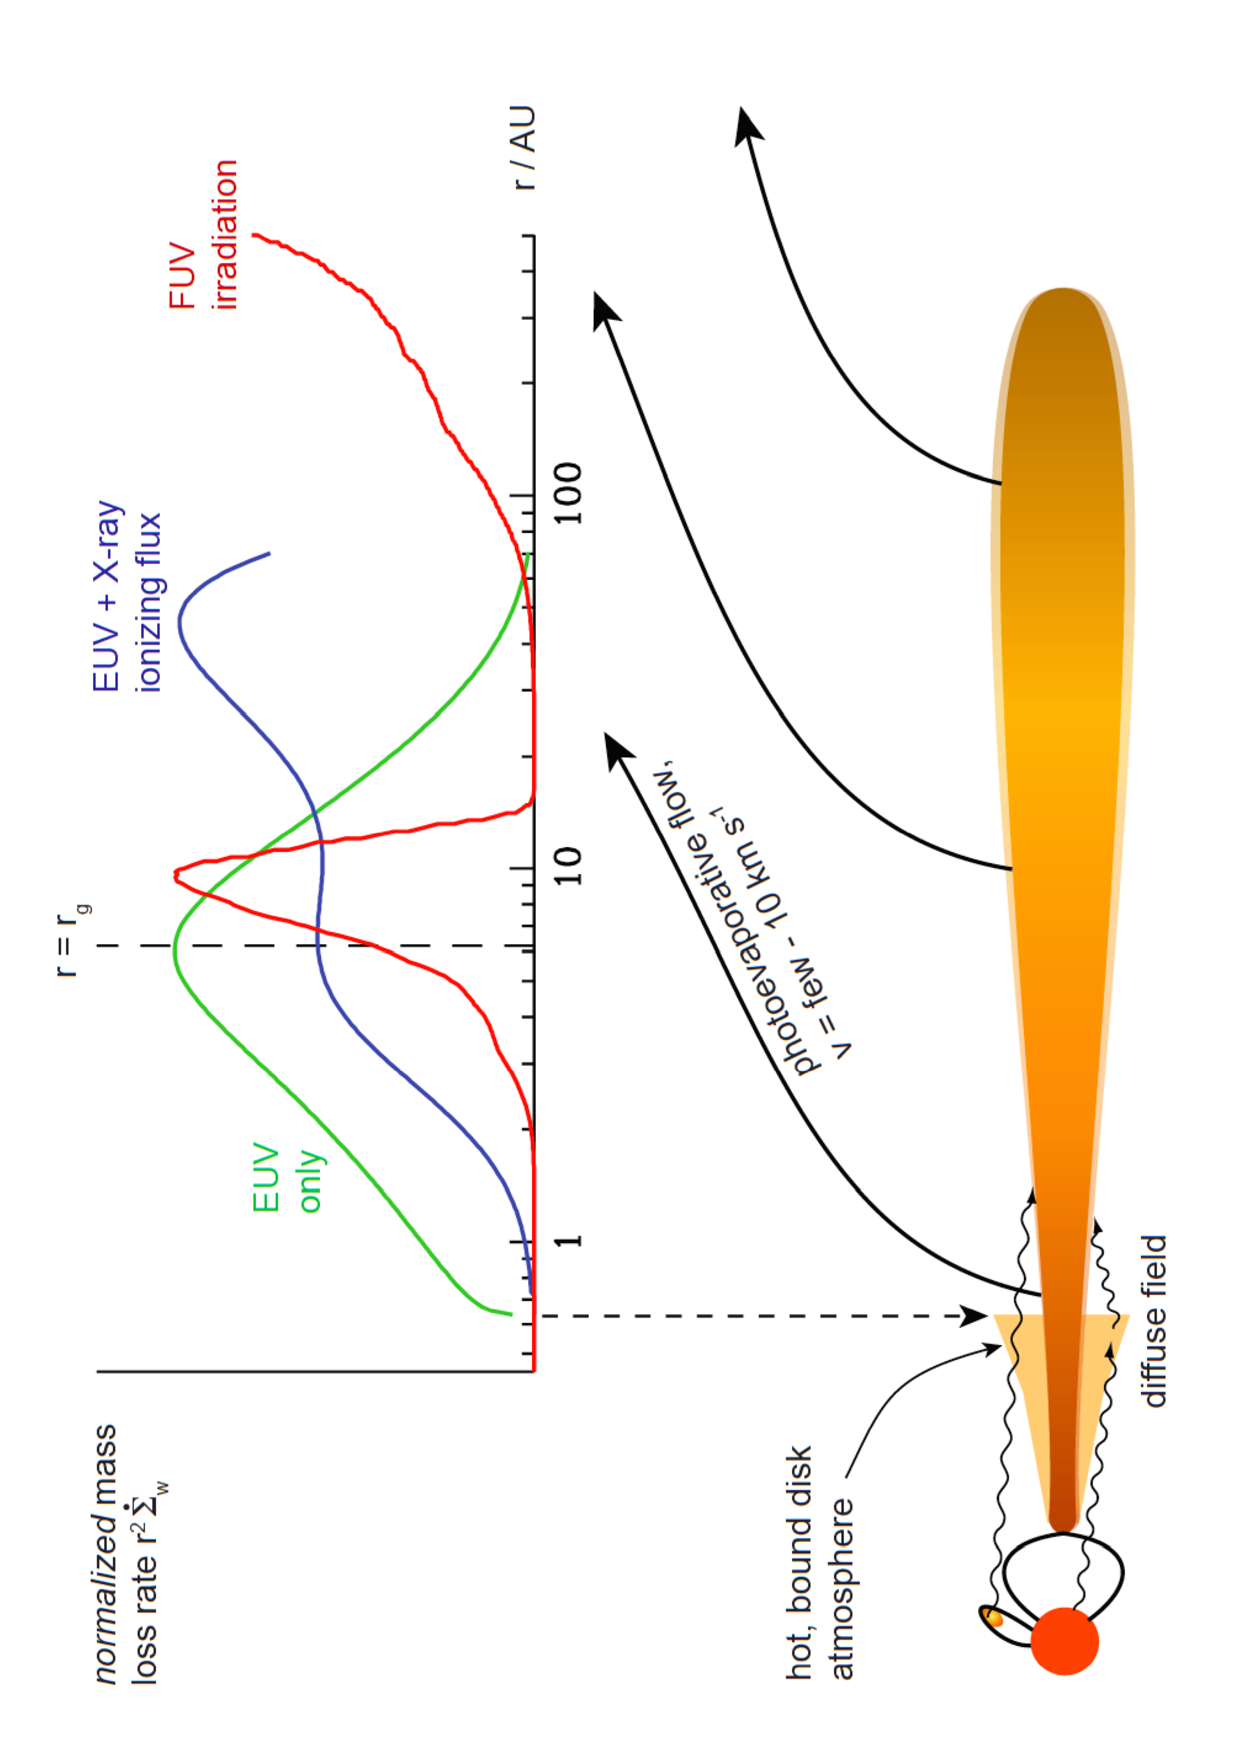
\includegraphics[width=0.75\linewidth, angle = 270]{profiles.pdf}
  \caption{From \citet{2011ARA&A..49..195A}. Different photoevaporation profiles
    corresponding to the EUV-only model of \citet{2006MNRAS.369..216A, 2006MNRAS.369..229A},
    the EUV+X-ray of \citet{2010MNRAS.401.1415O} and FUV model estimates of
    \citet{2009ApJ...705.1237G}. The profiles have been
    normalised, where the total mass loss rates can differ by over two
    orders of magnitude. }
  \label{fig:profiles}
\end{figure}


While the community now agrees on this broad brush picture,
quantitatively speaking, the dispersal mechanism is still largely
unconstrained. There is currently a hot debate in the literature as to
what type of radiation may be the main driver of the wind: Extreme-,
Far-UV or X-ray. This is a fundamental question as the mass-loss-rates
implied by the different models can differ by orders of
magnitudes. The mass loss rates determine the timescales of dispersal for
given initial disk conditions. The wind profile, i.e.\ the region of
the disk that is most affected by photoevaporation, is also very
different in each scenario 
\citep[e.g.][]{2014prpl.conf..475A, 2011ARA&A..49..195A}.
%(e.g.\ see Armitage 2011, Alexander et al. 2014). 
Figure~\ref{fig:profiles} shows the mass loss profile for the X-ray+EUV
\citep{2010MNRAS.401.1415O},
%(Owen, Ercolano et al. 2010),
EUV-only 
\citep{2004ApJ...607..890F}
%(Font et al. 2004) 
and FUV
%(Gorti, Dullemond \& Hollenbach 2009)
\citep{2009ApJ...705.1237G}
profiles. The X-ray profile is much
more extended than the EUV profile, which predicts mass loss only from
a vary narrow range of disk radii. The FUV model is again very
different, showing mass loss from the outer regions of the disk, hence
predicting in some cases an outside-in mode of dispersal. These
differences have important implications for the planet formation and
the migration 
process. For example, the total
mass loss rates in the disk sets the timescales for the formation of
gas giants, and together with the wind
profiles it sculpts the disk density distributions, profoundly affecting
the evolution of all planetary systems, by putting a stop to migration via
the formation of gaps in the gas. As an example, we have shown that
the photoevaporation profile strongly influences the final semi-major
axis distribution of exo-planets 
\citep{2015MNRAS.450.3008E}.
%(Ercolano \& Rosotti, 2015) 

While the importance of the final stages
of disk evolution to understand planet formation and explain the
diversity of exoplanets is largely recognised, a quantitative model describing this phase is
still lacking. The reason for that is that all current models are
somewhat 
incomplete. Some models focus on hydrodynamics and 
assume isothermal gas 
\citep[e.g.\ the EUV-only model of][]{2004ApJ...607..890F}
%(e.g.\ the EUV-olny model of Font et al. 2004), 
others focus on
chemistry but do not perform hydrodynamical calculations 
\citep[e.g.\ the FUV model of][]{2009ApJ...705.1237G}.
%(e.g.\ the FUV model of Gorti, Dullemond \& Hollenbach 2009). 
None of the existing models take into
account dust evolution in the underlying disk and entrainment of
grains in the wind. Together with James Owen, a former PhD student I co-supervised
at the Institute of Astronomy in Cambridge, I performed
the only existing radiation hydrodynamic calculations of X-ray  + EUV driven
winds to date 
\citep{2010MNRAS.401.1415O, 2011MNRAS.412...13O,
  2012MNRAS.422.1880O}. For this calculation
%(Owen, Ercolano et al. 2010, 2011a, 2012), 
we used realistic gas
temperatures obtained from X-ray photoionisation calculations
\citep{2008ApJ...688..398E, 2009ApJ...699.1639E}.
%(Ercolano et al. 2008, 2009). 
This led to a fundamental re-think to the
whole problem, as previous isothermal calculations had yielded much
lower mass loss rates (by two orders of magnitude). However, our
models, which still represents the state-of-the-art, also have
important limitations, since, most importantly, they do not include
chemistry and ignore the dust phase. Furthermore the resolution at
which the simulations were performed is insufficient to study lines with
emission regions extending close to the disk inner edge. The parameter
space covered by these models is also rather small. These
limitations make the application of current models to observations
impossible.  

As well as the uncertainties on mass loss rates and wind profiles,
which directly affect planet formation, there are also a number of
open questions regarding photoevaporation and the formation of the
observed TDs. A recent review by 
\citet{2016PASA...33....5O}
%Owen (2016) 
provides a discussion of
the current successes and problems of theoretical models in
explaining the origin and evolution of TDs. Here we will just list a
few issues that we believe should have priority in the development of a
quantitative theory which can be used to interpret observations. 

\begin{enumerate}
\item The observations of TDs have yet to reveal objects with large
  holes that do not accrete. Photoevaporation, however, predicts that a
  significant population of them should exist, unless the final
  removal is dominated by a fast run-away
  phase called ``thermal sweeping''. 
  \citep{2012MNRAS.422.1880O}.
% (Owen et al. 2012).
  The
  efficiency of  ``thermal sweeping'' has however recently been called
  into question 
  \citep{2016MNRAS.457.1905H}, however as will be discussed in more
  details below, a detailed calculation of thermal
  sweeping is still lacking. 
% (Haworth et al. 2016). 
\item The role played by FUV heating in the removal of the outer disk
  is unclear, due to the lack of hydrodynamical calculations that
  include this heating channel. FUV heating may provide a solution to the
 previous item, at least in some cases. 
\item Current estimates of the TD demographics as predicted by the X-ray
  model are based on extrapolations of the results with stellar mass
  and stellar emission properties. The validity of these
  extrapolations has yet to be proved. 
\end{enumerate}

\paragraph{Contribution of this team to the current state-of-the-art}

The first photoevaporation models developed were based on EUV
irradiation only. This was mainly due to the need of simplifying the
hydrodynamics by assuming an isothermal gas
\citep[]{2006MNRAS.369..216A, 2006MNRAS.369..229A}. 
An EUV heated gas, where
hydrogen is almost fully ionised, is indeed roughly isothermal
($\sim$10$^4$K), while the temperatures of a quasi-neutral X-ray
heated gas generally vary from a few hundred to a few thousand 
Kelvin. Here the hydrogen gas cannot directly be ionised by the X-ray
photons, 
thus it achieves only a very low level of ionisation, with the
exact ionisation level influencing the efficiency of the X-ray
heating. While the EUV-photoionisation process occurs of via the removal
of a single valence electron, X-rays generally remove an inner-shell
electron from a metal (e.g. C, N, O). The ejected supra-thermal electron produces then secondary
ionisations (of mostly H and He). A further complication is that multiple electrons may be
ejected as a consequence of inner shell ionisations, linking together
non-adjacent ionisation levels.

 The host of microphysics regulating
X-ray ionisation and heating is self-consistently included in the
three-dimensional photoionisation code MOCASSIN 
\citep{2003MNRAS.340.1136E, 2005MNRAS.362.1038E, 2008ApJS..175..534E}
%(Ercolano et al. 2003, 2005, 2008a) 
and has been applied to the X-ray photoionisation and
photoevaporation problem of protoplanetary disks 
\citep{2008ApJ...688..398E, 2009ApJ...699.1639E, 
2010MNRAS.406.1553E, 2016MNRAS.460.3472E, 
2010MNRAS.401.1415O, 2011MNRAS.412...13O, 2012MNRAS.422.1880O}
%(Ercolano et al. 2008b, 2009, 2010, 2016; Owen et al. 2010, 2011, 2012). 


In 
\citet{2008ApJ...688..398E, 2009ApJ...699.1639E}
%Ercolano et al. (2008b,2009)
the relevance of the X-ray photoevaporation process
to the dispersal of disks was proven for the first time. Indeed the mass
loss rates calculated were approximately two order of magnitude larger
than those previously obtained by the EUV-only model, able to compete
with observed accretion rates from T-Tauri stars. These early results
were based on hydrostatic calculations, which were later improved by
our 2D radiation-hydrodynamic calculations 
\citep{2010MNRAS.401.1415O, 2011MNRAS.412...13O, 2012MNRAS.422.1880O},
%(Owen, Ercolano et al. 2010, 2011, 2012), 
which still represent the state-of-the-art in
this field. This work also provided detailed mass-loss radial profiles
that have been used by us and others to study the photoevaporation
process in combination with planet formation in 1D and 2D
\citep[e.g.,][]{2013MNRAS.430.1392R, 2015MNRAS.454.2173R, 2015MNRAS.450.3008E}.
%(e.g.\ Rosotti, Ercolano et al. 2013, 2015; Ercolano et al. 2015). 

Over the last few years we explored several possibilities to test and refine our
models against observations. In 
\citet{2010MNRAS.406.1553E, 2016MNRAS.460.3472E}
%Ercolano \& Owen (2010, 2016)
and in
\citet{2010MNRAS.401.1636S}
%Schisano, Ercolano \& G\"udel (2010)
we
produced synthetic line profiles of forbidden transitions of heavy
metals observed in the optical and in the mid-infrared. We came to the
conclusion, however, that the strong temperature dependance of these
lines makes them unsuitable for use as wind diagnostics. 

In 
\citet{2010MNRAS.402.2735E}
%Ercolano \& Clarke (2010) 
we explored the metallicity dependance of the mass
loss rates, hoping for hints from disk statistics in several
regions. While available data support our predictions 
\citep{2009AIPC.1158..171Y, 2010ApJ...723L.113Y},
%(Yasui et al. 2009, 2010), 
these observations are challenging and have
remained sparse. The importance of the effects we noted in this
work for planet formation has however been widely recognised
\citep[e.g.,][]{2016arXiv161001170L}.
%(e.g.\ Lopez 2016). 

In 
\citet{2013MNRAS.434.3378O}
%Owen, Scaife \& Ercolano (2013)
we tested the models using
predictions at radio wavelengths. We were able to show in that work that our
observations of the famous transition disk around GM Aur were
consistent with our models, but could not really distinguish between
a EUV-only or an X-ray driven scenario. This line of work was however
used again by 
\citet{2014ApJ...795....1P}
%Pascucci et al. (2014)
to show that the EUV flux
impinging on protoplanetary disks is generally low, hence arguing
against a EUV-only model for dispersal. 

The work described in this section has provided the basis for many theoretical
and observational investigations, which cannot all be described
here. We will only finally mention our most recent application where
we were able to use our model to argue that the inner-most gap imaged
with ALMA by 
\citet{2016ApJ...820L..40A}
%Andrews et al. (2016)
in the disk around TW Hya, is
likely photoevaporative in origin 
\citep{2017MNRAS.464L..95E}.
%(Ercolano et al. 2017). 


\subsection{Project-related publications}

% Please list your own publications related to the proposed project, 
% adhering to the rules of the DFG guidelines 1.91. In brief, please note: 
% - Up to 10 publications
% - The work must be published or accepted.
% - Publications on astro-ph (arXive, SPIRES or articles with a DOI) count as published. 
% - Any work that is only in the status ``accepted'' MUST be attached to the proposal
%    together with the acceptance letter.
% - All publications in this section CAN be attached to the proposal. Please limit these
%    attachments to a minimum and please note that the reviewers may not read the attachments -
%    the proposal has to speak for itself.
% - The number of allowed publications refers to the sum of the publications listed
%    in ``1.1.1 Articles published or officially accepted by publication outlets...'' and 
%    in ``1.1.2 Other publications''. Publications which only exist on public repositories 
%    belong into the category ``Other Publications''.

%\subsubsection{
%Articles published or officially accepted by publication outlets with scientific quality assurance;
%book publications}

\begin{literature}

\item \textbf{Ercolano, B.},  Drake, J.; Raymond, J., Clarke, C.
  \textit{X-Ray-Irradiated Protoplanetary Disk Atmospheres. I. Predicted Emission-Line Spectrum and Photoevaporation}, 2008, ApJ
  688, 398. In this paper we use the MOCASSIN code to present a first
  estimate of the magnitude of the X-ray photoevaporation process in
  protoplanetary disks. We obtain mass loss rates that are
  significantly higher than previous estimates, showing
  the relevance of this process to the dispersal of disks. Before this work the
  importance of X-ray photoevaporation had not been recognised.  

\item \textbf{Ercolano, B.}, Clarke, C., Drake, J. \textit{X-Ray
    Irradiated Protoplanetary Disk Atmospheres. II. Predictions from
    Models in Hydrostatic Equilibrium}, 2009, ApJ 699, 1639. We
  further develop our models to include the feedback of X-ray heating
  on the disk-structure in hydrostatic equilibrium, and obtain more
  accurate estimates of the photoevaporation rates, which confirm our
  previous conclusions that the X-ray photoevaporation process is a
  main player in the dispersal of disks. These calculations provide the
  starting conditions for the full hydrodynamical investigations to
  Owen et al. (2010).

\item Owen J., \textbf{Ercolano B.}, Clarke,
  C. \textit{Radiation-hydrodynamic models of X-ray and EUV
    photoevaporating protoplanetary disks}, 2010, MNRAS, 
  401, 1415. We perform the first radiation-hydrodynamic calculations
  of an X-ray and EUV irradiated disk in 2D. For that we modified a
  standard hydrodynamics code (ZEUS-2D) to include the X-ray heating
  rates calculated in the previous papers (Ercolano et al. 2008, 2009). The rates obtained here
  for the standard model still represent the state of the art and are
  widely used in the community. 

\item \textbf{Ercolano B.}, Owen J. {\em Theoretical spectra of
    photoevaporating protoplanetary disks: an atlas of atomic and
    low-ionization emission lines}, 2010, MNRAS 406,1553. We postprocess the
  models of Owen et al. (2010) and obtain synthetic observations of
  atomic and low-ionisation emission lines to be compared with the
  observations. We show that our models compare favourably with the
  observations available at the time.

\item Owen J., \textbf{Ercolano B.}, Clarke C.  \textit{
  Protoplanetary disk evolution and dispersal: the implications of X-ray photoevaporation}, 2011, MNRAS, 412, 13.
  We explore the role of X-ray photoevaporation in the evolution and
  dispersal of viscously evolving T Tauri disks. Our models confirm
  that X-rays play a dominant role in the evolution and dispersal of
  protoplanetary disks giving rise to the observed diverse population
  of transition disks, including those with massive outer
  disks and with residual gas in their inner holes, which provides detectable accretion
  signatures.  

\item Owen J., Clarke \& \textbf{Ercolano B.}  \textit{On the theory of disk photoevaporation}
  2012, MNRAS, 422, 1880. We derive analytical scaling relations and
  derive estimates for the total mass-loss rates, as well as
  discussing the existence of similarity solutions for flows from
  primordial and transition disks. In this paper we catch a first
  glimpse at a new process for the clearing of the very last stages,
  which we name ``thermal sweeping''.

\item \textbf{Ercolano B.},Rosotti G. {\em The link between disk
    dispersal by photoevaporation and the semimajor axis distribution
    of exoplanets}, 2015, MNRAS 450,
  3008. We show here that details of the photoevaporation models
  (rates and profiles), strongly affect the planetary system
  configurations emerging from those disks. We suggest that the
  deserts and peaks seen in the distributions are a result of
  photoevaporation parking the giant planets at specific radii.

\item \textbf{Ercolano B.}, Owen J.  {\em Blueshifted [O I] lines from
    protoplanetary disks: the smoking gun of X-ray photoevaporation},
  2016, MNRAS 460. 3472
  We produce new synthetic observations of a particularly promising
  diagnostic, [OI] 6300 and demonstrate that the observations available at the
  time (before Simon et al. 2016) are consistent with the
  photoevaporation model. We show however that this line cannot be
  used to measure mass-loss-rates and suggest that a thermochemical
  model of the wind launching region is necessary. 

\item \textbf{Ercolano B.}, Rosotti G., Picogna G., Testi L.  {\em A photoevaporative gap in the closest planet-forming disk},
  2017, MNRAS 464L, 95
 In this letter we show that the innermost gap in the disk around TW
 Hya, recently imaged by Andrews et al. (2016) with ALMA, is very
 likely due to X-ray photoevaporation. We demonstrate how all current
 observational data fit the predictions of the model and provide new
 estimates for the timescales of dust-draining from the inner disk.

\item Keto E. and \textbf{Caselli P.}  \textit{The Different Structures of the Two Classes of Starless Cores}, 2008, ApJ
  683, 238. We construct a reduced chemical network for oxygen chemistry
   (including water and carbon monoxyde), include it into a
   hydrodynamical code of the evolution of Bonnor-Ebert (BE) spheres
   and compare the results with observations.  For the first time, we
   demonstrate that dense cloud cores contract as unstable
   quasi-equilibrium BE spheres, while the singular isothermal sphere
   and Larson-Penston solutions for dense core contraction do not
   reproduce the observed line profiles.  This was only
   computationally possible
   because the number of reactions was reduced to the core. A similar
   approach will be used in B1 and B2. 

\end{literature}


% \subsubsection{Other publications}
% 
% None 
% \subsubsection{Patents}
% 
% \paragraph{Pending}
% 
% None
% 
% \paragraph{Issued}
% 
% None

\section{Objectives and work programme}
\renewcommand{\leftmark}{\sc Objectives and work programme}


\subsection{Anticipated total duration of the project}

36 months

\subsection{Objectives}


\connect{The overarching aim of this project, in common with projects B2 (PI
Caselli \& Ercolano) and C2 (PI Ercolano),
is to identify new wind tracers and use them to constrain mass loss rates and hence
disk dispersal models, leading to the formation and evolution of Type 1
transition disks. 

The new comprehensive radiation-hydrodynamics photoevaporation models
developed in this project will enable a quantitative
spectroscopic evaluation of new diagnostics of disk winds, via
detailed astrochemical models developed together with project B2,
using the dust model for the wind and atmosphere from project C2. }

We will perform a comparison between TDs and
primordial disk to provide important constraints on the wind
architecture and the mechanism driving the dispersal. 
Type 1 TDs, are particularly interesting as the streamline architecture of their winds
and the profiles of the lines that are produced in the wind
differ from those of primordial disks. (e.g.\ Ercolano \& Owen
2010, Ercolano \& Pascucci, 2017, in prep.). Indeed the lines
are expected to be broader and brighter for e.g.\ inner cavities of a few to 10 AUs.  

The immediate objective of project B1 is to produce a new set of
X-ray+UV photoevaporation models which goes well beyond the current
state-of-the-art, described in the previous section. 

\connect{The new models will constitute the backbone for the joint
investigation to be carried out in projects B2 and C2}, as well as
allowing us to address the following important unsolved questions in
the formation of Type 1 transition disks and their further evolution: 

\begin{enumerate}
\item How fast do Type 1 TDs evolve/disappear after the inner disk has
  drained?
\item How does the formation \& evolution of Type 1 TDs scale with
  stellar mass and stellar emission properties?
\item What is the role of FUV heating in the late evolution of Type 1
  transition disks? 
\end{enumerate}

%{Test whether Type 2 TDs (large holes, large accretion rates) may
%result from radiative transfer effects on a tilted inner disc. This
%idea stems from  the recent suggestion (e.g.\ Marino et al. 2015, Montesino et
%al. 2016) that some Type 2 TDs may have a tilted inner disc. 
%A tilted inner disk may strongly influence photoevaporation by
%allowing radiation to reach outer disk regions and may produce the
%large inner holes of (some) Type 2 TDs. This is certainly a worthwhile
%new challenge requiring the development of 3D simulations.  }

%{\color{red} the marino and montesino idea must also be included in
 % the intro and also in the background section of this proposal}




\subsection{Work programme including proposed research methods}
% for each applicant
In this project we will construct a
library of high resolution X-ray+EUV wind solutions for an extended grid of
X-ray luminosities and stellar masses, covering all observed
values. Our new calculations will make use of a new temperature
scheme (Ercolano, Picogna \& Owen, 2017, in prep.), derived from
new more extensive X-ray + EUV photoionisation models.  The new
temperature scheme
significantly reduces the error at low ionisation parameter values,
allowing us to make solid predictions of the late evolution of
transition disks. 

Furthermore, our previous calculations 
\citep{2010MNRAS.401.1415O, 2011MNRAS.412...13O, 2012MNRAS.422.1880O},
%(Owen et al. 2010, 2011, 2012)
could only account for heating 
in the ionised phase of the wind, ignoring that the region beyond the
layer heated by the soft X-ray ($<1keV$) which could be heated by FUV
radiation with typical PDR or XDR characteristics. While we show in
\citet{2012MNRAS.422.1880O},
%Owen et al. (2012), 
that this should not affect the mass loss rates at
around 1-10~AU, the effect of FUV heating at larger radii may be
important. This is particularly relevant to the late evolution of
transition disks, when the cavity becomes larger than approximately
30~AU. Indeed one of the
problems with current photoevaporation models is the prediction of a
large number of non-accreting transition disks with large holes
\citep[e.g.,][]{2016PASA...33....5O}.
%(e.g.\ Owen 2016). 
In this project we will be able to test the
suggestion that FUV heating may take over the late-stage evolution of
transition disks, speeding up their final complete erosion. 

%We have recently coupled our 3D X-ray and EUV Monte Carlo photoionisation
%code MOCASSIN to the KROME package to solve the chemistry in the
%deeper layers of the disk (Ercolano \& Grassi, 2017, in
%preparation). The code has been benchmarked for a simple toy network,
%but we will need input from project B2 to include an appropriate
%network to model this region and devise a new temperature scheme to
%include in our radiation-hydrodynamic simulations.   


\subsubsection{Research Tools}

For this project we will need the following tools: 
\begin{enumerate}
\item A hydrodynamical code modified to include the
  effects of X-ray + EUV irradiation as we did in 
  \citet{2010MNRAS.401.1415O}.
%Owen et al. (2010). 
  For
  that we use the Pluto code, for which extensive expertise
  exists in our team and in other teams of this Research Unit (e.g. D1
  \& D2 -- Applicants Kley \& Dullemond).
\item An efficient astrochemistry package to include a reduced
  chemical network into PLUTO. For that we will use KROME 
  \citep{2014MNRAS.439.2386G}  
%(Grassi et al. 2014) 
and link it with PLUTO. Dr Grassi will take active part in helping
with the implementation of the algorithm.
\item An efficient radiative transfer algorithm to model the region
  just beyond the X-ray dominated region. We can use initially the
  implementation of radiative transfer and stellar irradiation
for the PLUTO code 
\citep{2013A&A...559A..80K},
%(Kolb et al., 2013), 
developed by the group of Kley
(PI of project D2). If this is proved not to be sufficient for our
aims, the Applicant also has experience in the
development of hybrid algorithms  
\citep{2014ASSP...36..127O}.
%(Owen, Ercolano \& Clarke 2014). 

% A photoionisation and chemical code which includes X-ray
 % heating and ionisation to obtain a new comprehensive temperature
 % scheme for the radiation-hydrodynamic simulations. The Applicant is the
 % author of the 3D Monte Carlo photoionisation and dust radiative
  %transfer code MOCASSIN (Ercolano et al. 2003, 2005, 2008b),
 % which has already been used to calculate the 
 % emission line spectra from the ionic phase of X-ray winds (Ercolano
 % \& Owen 2010; 2016). The code has
 % now been coupled and benchmarked to the KROME code to perform
 % arbitrary chemical calculations (Ercolano \& Grassi 2017, in prep)
 % and needs now only the appropriate chemical network, which
 % we will obtain from project B2.  
\end{enumerate}

\subsubsection{Research Plan} 


\begin{figure}
\centering
\begin{minipage}[b]{.47\textwidth}
  \centering
  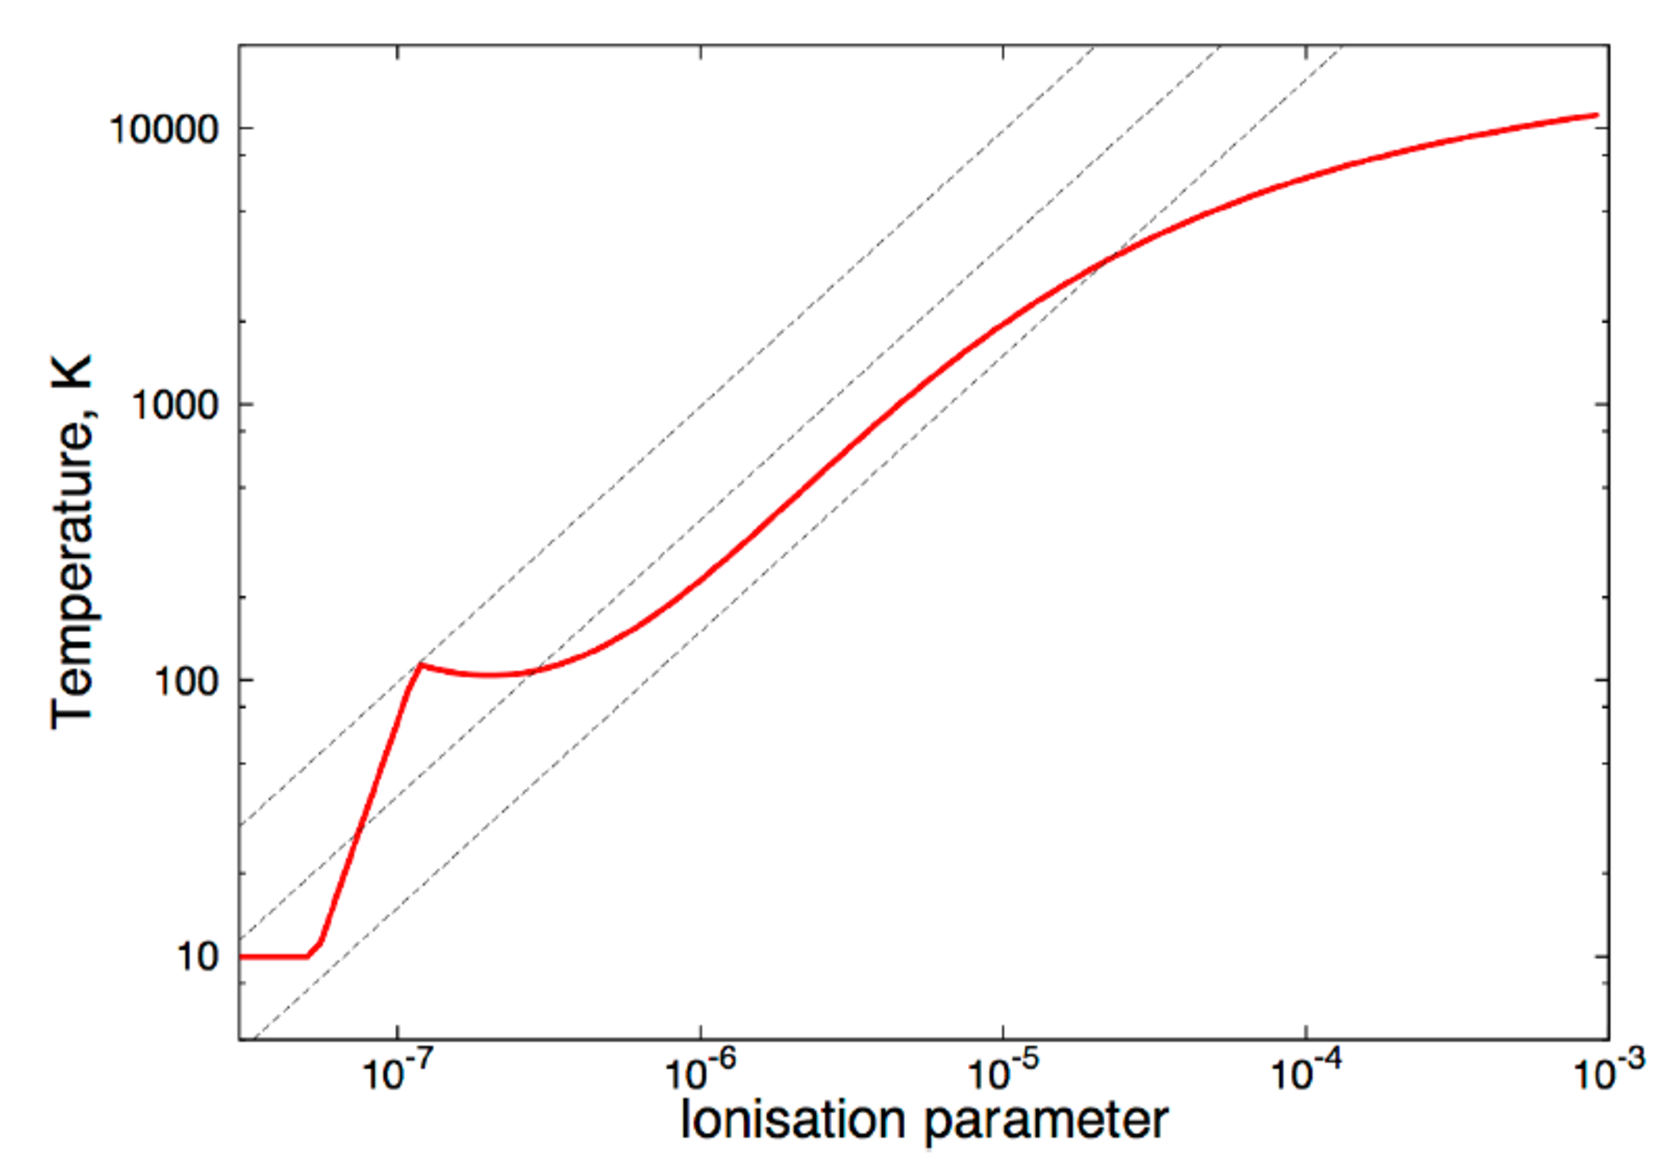
\includegraphics[width=0.95\linewidth]{xite_a.pdf}
\end{minipage}%
\hspace{0.05\textwidth}
\begin{minipage}[b]{.47\textwidth}
  \centering
  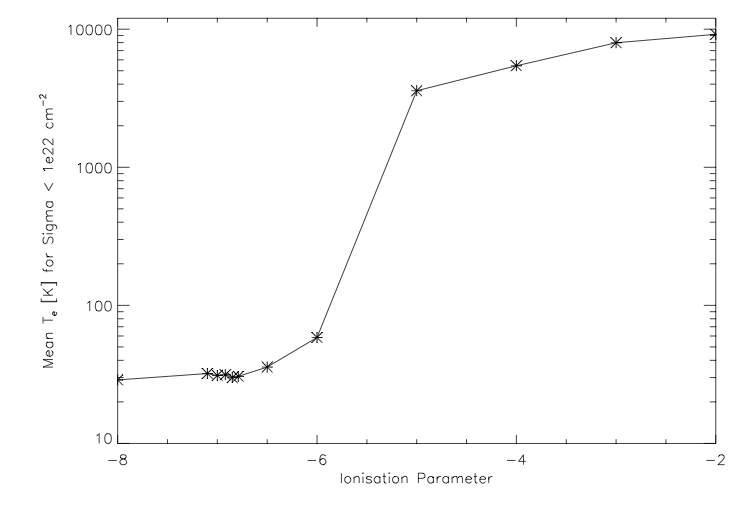
\includegraphics[width=\linewidth]{a.png}
\end{minipage}
\caption{The electron temperature versus ionisation parameter relation
in the calculations of Haworth et al. (2016), \caphighlight{left panel}, compared to
our most recent calculations Ercolano, Picogna \& Owen, (in
preparation), \caphighlight{right panel}.}
  \label{fig:xite}
\end{figure}




\paragraph{Preparatory work}

In this section we will describe
preparatory work that is currently being carried out by Dr
Picogna. Dr Picogna is currently employed in the group of Prof. Ercolano via
an Excellent Initiative grant from the LMU, awarded to the Applicant to carry
out preparatory work for this Research Unit proposal. The grant, which
was extended using funds from the faculty will end in November
2017. 

The determination of gas temperatures in a photoionised gas, in a
photodissociation region (PDR) or in an X-ray dissociated region (XDR)
is computationally expensive. It requires, first of all 
performing a radiative transfer (RT) calculation in order to determine the
radiation field at each point of the region. Then matrices of thermal and
ionisation balance and/or rate equations have to be solved. The RT and
the balance/rate equation are often coupled through the
temperature-dependent gas opacities, and one needs to iterate to
obtain a solution. There is a host of microphysics
that needs to be taken into account, last but not least the thermal
coupling of the gas and the dust phase. Even an extremely simplified
version of the above has large computational costs, if it needs to be performed at
every time-step of a hydrodynamical calculation. 

In such cases it is convenient to look for parameterisations of the
gas temperature in terms of quantities that are easy to determine on
the fly during the hydrodynamical run (e.g.\ gas properties and/or column density). 
Indeed the radiation-hydrodynamical calculations of X-ray + EUV driven
photoevaporative winds of 
\citet{2010MNRAS.401.1415O, 2011MNRAS.412...13O, 2012MNRAS.422.1880O},
%(Owen et al. 2010, 2011, 2012), 
described in the previous section, were performed
using such a temperature paremeterisation. The parameterisation was
determined via detailed X-ray photoevaporation models using the
MOCASSIN code 
\citep{2008ApJ...688..398E, 2009ApJ...699.1639E}
%(Ercolano et al. 2008, 2009)
The models were run with a version of the {\sc
  zeus2d} code which was modified by us to include a temperature
scheme based on the ionisation parameter at each cell in the
calculation. 
This was based on our previous work 
\citep{2008ApJ...688..398E, 2009ApJ...699.1639E}.
%Ercolano et al. (2008, 2009). 
where it was shown that, within the
penetration depth of $\sim$1keV X-rays ($\sim 10^{22}cm^{-2}$), the
temperature of a parcel of gas with hydrogen number density, $n_H$, at
distance $r$ from the central star, could be roughly approximated by a
function of the ionisation parameter, defined as $L_X/(r^2 n_H)$,
where$L_X$ is the stellar X-ray luminosity. The error on the
temperature was found to be small for high ionisation parameter values, but it
becomes systematically larger at the low end. 

As the gas temperature enters the hydrodynamics via the square root
dependance in the sound speed, the small error at high values of the
ionisation parameter, typical for the regions where the bulk of the
wind is driven from in primordial disks, is unlikely to produce large
uncertainties in the mass loss rates. For more evolved objects, like
transition disks in the phase of final dispersal, however, the ionisation
parameter decreases dramatically as the cavity becomes larger. The
evolution of transition disks depends thus sensitively on the temperature
of the gas at low ionisation parameters, which is currently poorly
represented by the parameterisation of 
\citet{2008ApJ...688..398E, 2009ApJ...699.1639E}.
% Ercolano et al. (2008, 2009). 
Note that the recent work of 
\citet{2016MNRAS.457.1905H},
%Haworth, Clarke \& Owen (2016), 
presents a form of the temperature ionisation parameter relation which is incorrect at
low values of the ionisation parameter. The kink at ionisation
parameters just above $10^{-7}$ (left panel of Figure~\ref{fig:xite}) is an artefact of their implementation
of the photoionisation models. We have recently performed new detailed
photoionisation calculations and obtained the curve shown in the right
panel of Figure~\ref{fig:xite} (Ercolano, Picogna \& Owen, 2017, in prep.).
Figure~\ref{fig:xite} shows no kink in the temperature parameterisation at
low ionisation parameter, which is important as some of the
conclusions reached by
\citet{2016MNRAS.457.1905H} are a consequence of this kink.  Our
collaborators J. Owen and C. Clarke, as well as the first author, Dr Haworth, have been informed of the problem
and agree with our more recent calculations. Furthermore we have now
found a more accurate scheme that allows us to reduce the error on the
temperature by taking into account the gas column density as an additional
parameter. 

As well as the major shortcoming highlighted above, the Owen et
al. (2010) calculations which were used to make predictions on
the ionised phase of the wind spectra 
\citep{2010MNRAS.406.1553E, 2016MNRAS.460.3472E},
%(Ercolano \& Owen 2010; Ercolano \& Owen 2016), 
suffered from low spatial resolution,
precluding us from being able to model the inner region of the bound disk, which
may be relevant to interpret the broad wings of some of the
wind-tracing emission lines presented in the recent
work of 
\citet{2016ApJ...831..169S}.
%Simon et al. (2016). 
Furthermore, a very limited
parameter space was investigated, which included only two values for
stellar mass, 3 values of X-ray luminosity for primordial disks and a
single stellar mass and X-ray luminosity value for transition disks
with 3 values for the cavity radius. This is not enough to draw 
significant conclusions about trends in possible wind diagnostics. 

In this project we aim at constructing new photoionisation models to
remedy the shortcoming of the current models highlighted above. To
that aim we have modified the hydrodynamical code PLUTO 
\citep{2007ApJS..170..228M, 2012A&A...545A.152M}
%(Mignone et al. 2007, 2012) 
to include the
effects of X-ray and EUV irradiation using the temperature-ionisation
parameter from 
\citet{2008ApJ...688..398E, 2009ApJ...699.1639E}
%Ercolano et al. (2008,2009) 
also employed by 
\citet{2010MNRAS.401.1415O}
%Owen et al. (2010)
for the ZEUS2D calculations. We have implemented the
standard scheme in order to be able to compare our wind solutions to 
those available for a 0.7 and 0.1 M$_\odot$ central
stars 
\citep{2010MNRAS.401.1415O, 2011MNRAS.412...13O, 2012MNRAS.422.1880O},
%(Owen et al. 2010, 2011, 2012), 
for similar spatial
resolution. This will ensure that we have implemented the algorithm
correctly in PLUTO, before we move on with project B1 and implement
the improved temperature scheme. 



\begin{figure}
  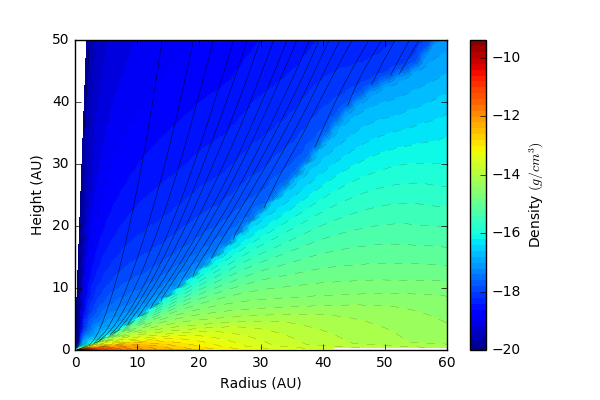
\includegraphics[width=0.85\linewidth]{streamlines.png}
  \caption{Column density map of our PLUTO simulation of the standard
    model from Owen et al. (2010), i.e. a 0.7 M$_{\odot}$ star with
X-ray luminosity of 2$\times 10^{30} erg/sec$. The figure is in polar coordinate,
    where the colour scale indicates column density and the overlain
    black lines are the streamlines tracing the outflow. }
  \label{fig:streamlines}
\end{figure}



\begin{figure}
  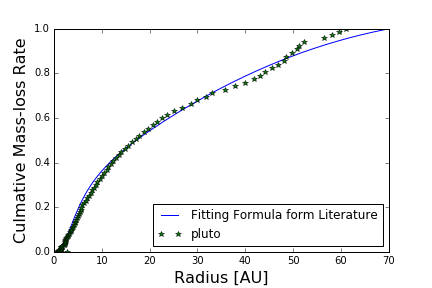
\includegraphics[width=0.85\linewidth]{cmdot_compare.png}
%  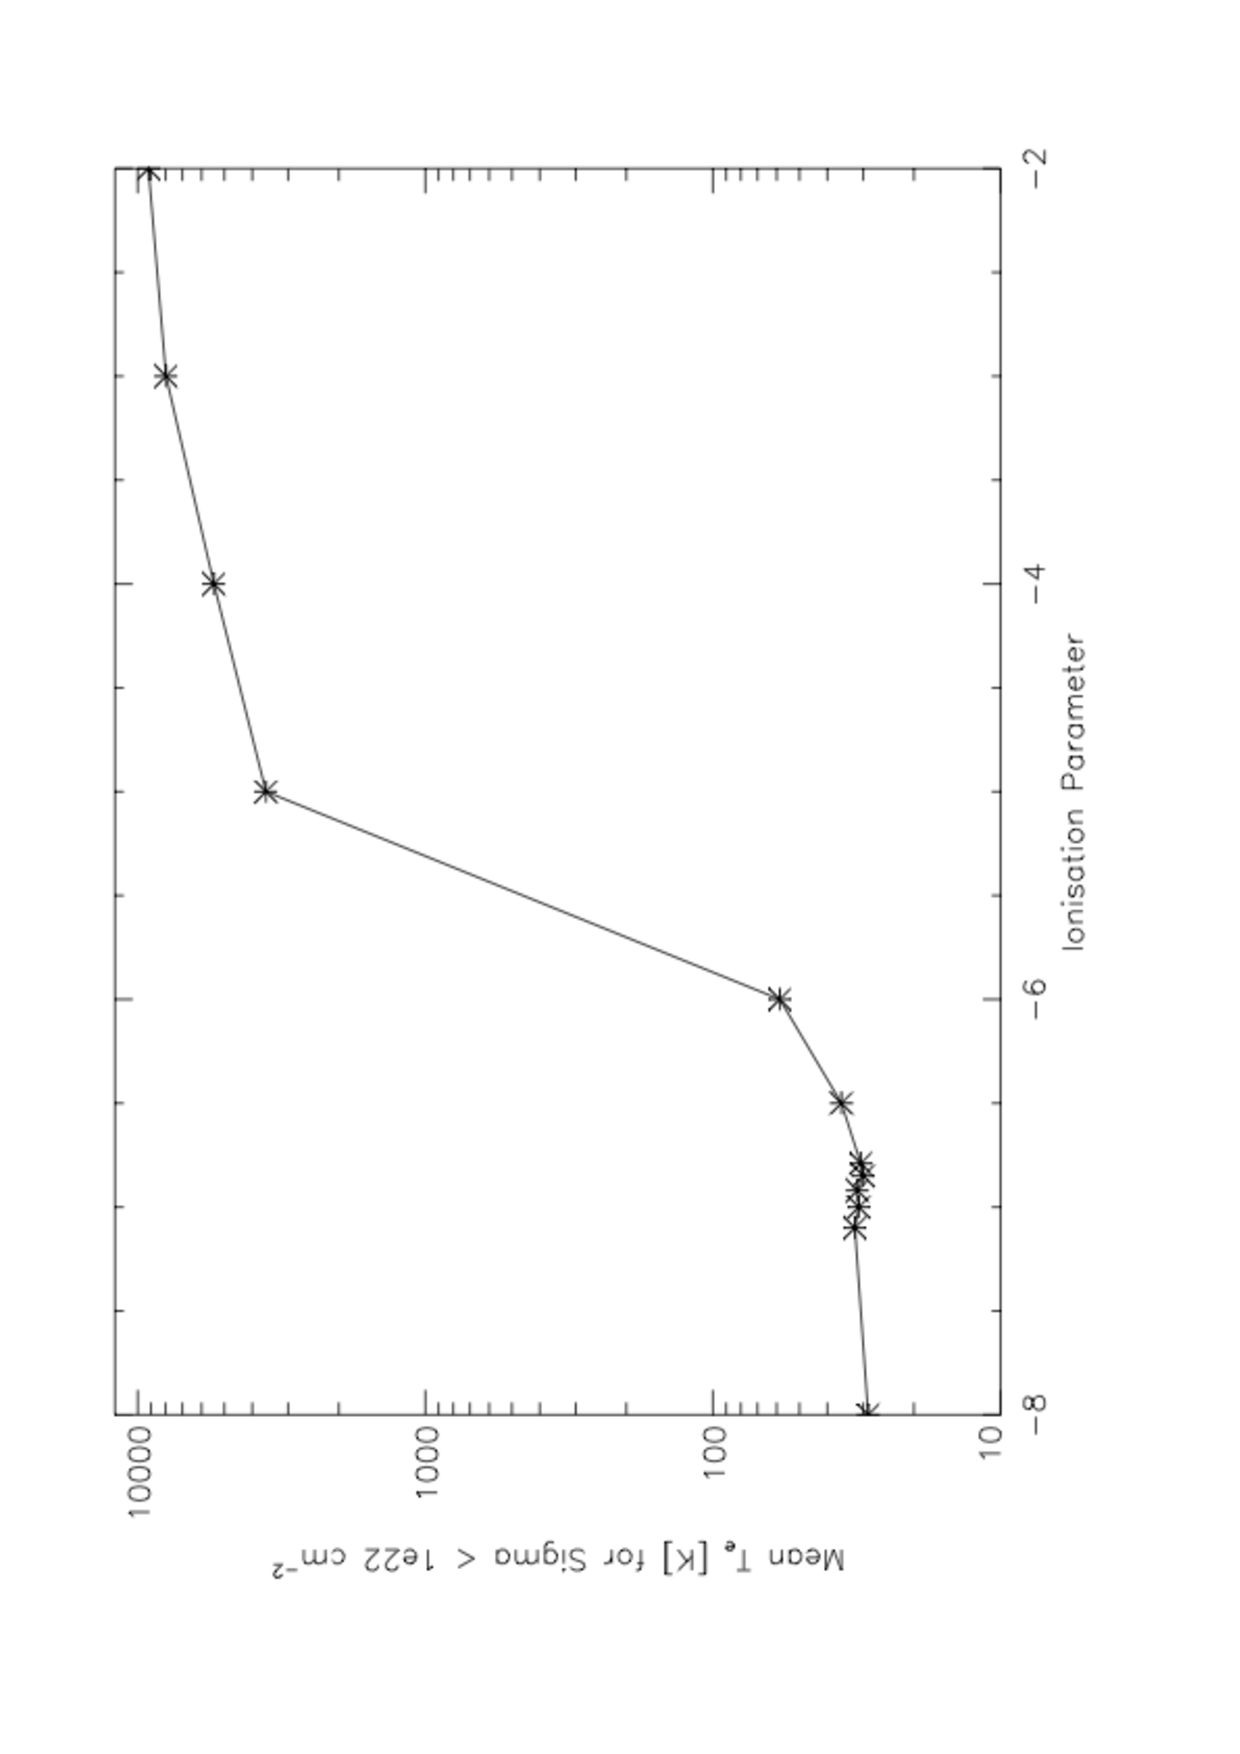
\includegraphics[width=0.35\linewidth, angle =
%  270]{cumsigmadot.pdf}
%  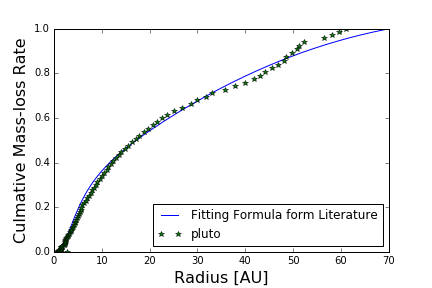
\includegraphics[width=0.45\linewidth]{cmdot_compare.png}
  \caption{The cumulative mass-loss-rate
    as a function of disk radius from the PLUTO calculation (green
    stars) is compared to the fitting formula (solid blue line) obtained from the
    literature (Owen et al. 2010). The integrated value (to 100 AU) of the
    mass loss rate is approximately 1.2$\times 10^{-8} M_{\odot}/yr$.}
 \label{fig:sigmadot}
\end{figure}


Figure\ref{fig:streamlines} shows a snapshot from our most recent simulation
with our modified version of PLUTO 
aiming at reproducing the standard model of
\citet{2010MNRAS.401.1415O}. This is for 0.7 M$_{\odot}$ star with
X-ray luminosity of 2$\times 10^{30} erg/sec$. For further details on
the simulation set-up we refer to \citet{2010MNRAS.401.1415O}. The
figure shows column densities in a quarter of the disk in
two-dimensional polar
coordinates. Overplotted black lines are streamlines showing the
outflowing gas. As mentioned above, in order to test that our implementation of the
temperature scheme works correctly we have used the same
parameterisation used by 
\citet{2010MNRAS.401.1415O}. 

We match the global
mass-loss-rate to within 15\% (we obtain a value of 1.2$\times 10^{-8}
M_{\odot}/yr$ and we can
reproduce the approximate wind profile, shown in
Figure~\ref{fig:sigmadot}. This plot shows the cumulative mass-loss-rate
    as a function of disk radius from the PLUTO calculation (green
    stars), compared to the fitting formula (solid blue line) obtained
    from the     literature (Owen et al. 2010). 

\subsubsection{Months 1-12}
In the preparatory work described in the previous section we have
implemented the standard temperature scheme from 
\citet{2008ApJ...688..398E, 2009ApJ...699.1639E}
%Ercolano et al.\ (2008, 2009) 
into PLUTO and have benchmarked the results against
the work of 
\citet{2010MNRAS.401.1415O}.
%Owen et al.\ (2010). 
In the first 12 months of the Research
Unit we will then proceed with the implementation of the new, more accurate
temperature scheme described in the previous Section (Ercolano,
Picogna \& Owen, 2017, in prep.). We will compare the resulting
wind rates and profiles for the primordial and transition disk
case presented by Owen et al. (2010). While we do not foresee large
changes in the rates for primordial disks, as described in the
previous section the evolution of transition disks will be most 
likely affected. 

In particular we will test the late evolution of transition disks to
estimate whether there is a radius for the inner cavity at which
photoevaporation stalls. In that case one would expect to be able to
observe a population of transition disks with large cavity and no
accretion signature (relic disks), which to date remains elusive. A solution to this
problem, form the theoretical stand-point, would be the triggering of
a fast final clearing phase, as the proposed final thermal sweeping
(Owen et al. 2011). Our models will be able to test this hypothesis in
detail for the first time, as previous works have all been limited by
the uncertainties in the temperature parameterisation of the X-rays at
low ionisation parameters (e.g. Haworth et al 2016). \connect{We will then
create synthetic transition disk population to check the occurrence of relic disks and
compare it with the limits shown by current observational surveys from
which we will be informed by the A1 team. }

Furthermore, the new models will have much higher spatial
resolution extending much closer into the star, in order to allow
tracking the profile components of emission line which may be produced from the inner bound
atmosphere of the disk (see discussion in Ercolano \& Owen 2016 and in
the Introductory section of this proposal).

\connect{This first set of models for $\sim$solar mass stars at a typical X-ray
luminosity ($\sim 10^{30}$erg/sec) will be then passed on to projects
C2 and B2 for the dust and detailed chemistry calculations. }

\subsubsection{Months 13-24}

Once our machinery is complete and well-tested we will be able to
switch to production-mode and extend significantly the parameter space
of the calculations. Specifically, we will vary the mass of the central star and its X-ray
luminosity as well as the accretion properties of the
disk. Furthermore models of transitions disks at several stages 
of evolution, as tracked by the radius of their inner cavity, will be
performed. 

\connect{As new models become available and we populate the parameter space, we
will make the grids available immediately to projects C2 and B2 for
the dust and detailed chemistry calculations. At this stage we will
already start to regularly check our model predictions against
observations, with the help of experts from projects A1 and A2. }

The new models will also allow us to investigate how
the photoevaporation process scales with stellar mass and stellar emission
properties. We will test the theoretical relations for X-ray photoevaporation 
predicted by means of semi-analytical models and ab-initio arguments
by Owen et al.\ (2012). These relations are already being widely used in
the literature and they are a crucial ingredient for population
synthesis models of planet formation, where photoevaporation is
included in the disk evolution and affects the timescales and location for
the formation of giant planets, as well as their successive
migration. 

The larger parameter space will also allow us to improve on our
initial calculations to construct more accurate synthetic
populations of evolved disks to match
the observed demographics of Type 1 TDs. \connect{Note that project A1 will
keep an up-to-date record of the transition disk demographics
throughout the duration of the Research Unit. } \\

\subsubsection{Months 25-36} 
The role of FUV heating in supporting or competing with the X-rays in
the removal of the disk is still uncertain. As we discussed in the
previous sections, the work of Gorti, Dullemond \& Hollenbach
(2009), based on 1+1D thermochemical calculations in hydrostatic
equilibrium, suggest that a vigorous thermal wind may be driven as a
result of FUV-heating. For some disk parameters (in particular in the
presence of PAHs), the FUV is shown to reach mass-loss-rates
comparable to those driven by X-rays. An hydrodynamical calculation of
an FUV driven wind is however still lacking and it is urgently needed
in order to assess the importance of this process, in particular at
large disk radii, which is relevant to the problem of disk relics,
amongst other things. 

\connect{At this stage of the Research Unit a robust and well tested
  reduced chemical network should be available from project B2 (PI
  Caselli, Ercolano). We will now couple our modified version of the
  PLUTO code to the KROME package to solve the chemistry using the
  reduced network from B2 and obtain the temperatures of the gas on
  the fly in the regions beyond the X-ray dominated regions.} For 
that we will receive help from our collaborator Dr.\ Grassi, who is the main
developer of the KROME code. Dr.\ Picogna has already attended the KROME
school this year (\url{http://kromepackage.org/bootcamp/}) and a simple
feasibility test has shown that this is a realistic task. As an example,
KROME is already implemented in a number of hydrodynamics codes (e.g.\ {\sc
  ramses, enzo, flash, gasoline, gizmo}). A number of publications performed
with these codes are listed on the KROME webpage
(\url{http://www.kromepackage.org/}).

A streamlined form of radiative transfer
will be needed in PLUTO at this point, meaning that these calculations will
probably be expensive to run.  This is however necessary in order to
estimate the value of the  FUV field reaching different regions of the
disk atmosphere, where the optical depth are not high enough to
justify the use of a  (grey) flux limited diffusion method.
Implementation of an efficient radiative transfer algorithm in PLUTO
will be carried out together with the Applicant who has experience in the
development of hybrid algorythms 
\citep[e.g.,][]{2014ASSP...36..127O}.
\connect{A simple RT scheme is
already available for PLUTO 
\citep{2013A&A...559A..80K},
%(Kolb et al.\ 2013), 
which was developed in
the group of our Prof.\ Kley (PI from project D1). Hence there is
a substantial body of experience within our Research Unit team to
successfully perform this task.}

Note that we do not plan to run a full
parameter space grid including the effects of the FUV heating. 
Our simulations will be limited to a selected number of cases
aimed at specifically testing how strongly, and for what initial
conditions, FUV heating may affect the evolution of the outer regions
of disks, in particular of those in transition.\\

\subsubsection{Future Outlook}

A natural further step of this work is to perform a small set of 3D
simulations to explore the effects of asymmetries in the inner
disk and/or the presence of giant planets in the disk. We expect to
see dramatic effects in the photoevaporation 
profile and in the wind architecture, which may lead to the formation
of large hole TDs. This avenue has never been explored before and,
while these models come at severe computational costs, they are likely to provide us
with important insights on the structure and origin of TDs. 

\connect{In particular in the second funding period of the Research
  Unit, the results from projects D1 and D2 will be available to
  us, and the natural further step will be to combine photoevaporation
to planet-disk interaction calculations. }


\subsection{Data handling}

A library of the hydrodynamical solutions in steady state (gas density
and velocity)  will be shared initially amongst the Research Unit
members only and will be made available online on the public partition
of the Research Unit server at the end of the first funding period. 

\subsection{Other information}
% Please use this section for any additional information you feel is
% relevant which has not been provided elsewhere.

Not Relevant

\subsection{Information on scientific and financial involvement of international cooperation partners}

Not Relevant

\section{Bibliography}

\begingroup
\renewcommand{\section}[2]{}%
\bibliographystyle{aa}
\bibliography{B1}
\endgroup


\section{Requested modules/funds}
\renewcommand{\leftmark}{\sc  Requested modules/funds}
% Explain each item for each applicant (stating last name, first name).

\subsection{Basic Module}

\subsubsection{Funding for Staff}
% Please note that funds for your own temporary position (“Eigene Stelleâ€)
% are not to be included here; this belongs to the separate “Module Temporary Positionâ€.

We require funding for one Postdoc to work at the LMU in the group of
Prof.\ Ercolano. In case of an award Dr Picogna has expressed interest
in taking on the post. Dr Picogna is currently employed in the group of the
PI and is performing preparatory work for the project. Dr Picogna's
expertise in astrophysical fluid dynamics and his familiarity with the
subject is of great advantage for the achievement of the aims of this
project. Dr Picogna's contract ends in November 2017.

\subsubsection{Direct Project Costs}


\paragraph{Equipment up to EUR 10,000, Software and Consumables}

Theoretical numerical research can only be done when sufficient and
appropriate computational facilities are available. While production
runs will be done on supercomputer facilities, a substantial part of
the work in this project is code development. Testing these codes on
realistic problems requires a workstation for the postdoc -- which is
beyond the standard base equipment 
(Grundausstattung). We therefore request a workstation-grade desktop
computer for the postdoc position for \EUR{3 000}.

\paragraph{Travel Expenses}

% Total: 17400 \EUR{} Justification : 
% Each year one national trip (meeting of Astronomical Society, national
% meetings) and one international trip (conference, visit
% collaborators) for the postdoc and the Applicant. 
% 
% 
% Cost estimate: 
% \begin{itemize}
% \item National trip: 5 overnight stays, train/airfare,
% conference fee; 1000 \EUR{} (6000 in total over 3 years).
% \item International trip: 6 overnight stays, airfare, conference fee;
%   1500 \EUR{} (9000 total over 3 years).
% \end{itemize}

Travel within the Research Unit is handled in project Z. In addition we
request funding for conference travel for the personnel and one Applicant.
This includes one national (1.000 \EUR{}) and one international (1.500 \EUR{})
conference trip per year, totalling 2.500 \EUR{} per person per year. 

For this project this totals 5.000 \EUR{} per year for the postdoc
and one Applicant, which is in total 15.000 \EUR{}.



\paragraph{Visiting Researchers (excluding Mercator Fellows)}

During the course of the project a one week long visits to our main
international collaborator, Dr J.~Owen (currently at Princeton
University, will move to Imperial College London in 2017).
This includes airfare and 6 overnight stay 1200 \EUR{}

\paragraph{Other Costs}

None

\paragraph{Project-related publication expenses}

We request \EUR{750} per year (a total of \EUR{2 250}) for publication
expenses, mainly to support open access options or whenever necessary,
publication in non-free journals.

\subsubsection{Instrumentation}

None 

\paragraph{Equipment exceeding EUR 10,000} 

None

\paragraph{Major Instrumentation exceeding EUR 100,000} 

None 

% \subsection{Module Temporary Position}
% 
% Not Relevant
% 
% \subsection{Module Replacement Funding}
% 
% Not Relevant
% 
% \subsection{Module Mercator Fellows}
% 
% Not Relevant
% 
% \subsection{Module Public Relations Funding}
% 
% Not Relevant

\section{Project requirements}
\renewcommand{\leftmark}{\sc Project requirements}

\subsection{Employment status information}
% For each applicant, state the last name, first name, and employment
% status (including duration of contract and funding body, if on a
% fixed-term contract).

Barbara Ercolano, Professor at the Ludwig-Maximilians-Universit\"at
M\"unchen  (permanent)

\subsection{First-time proposal data}
% Only if applicable: Last name, first name of first-time applicant.

Not Relevant

\subsection{Composition of the project group}
% List only those individuals who will work on the project but will not
% be paid out of the project funds. State each person’s name, academic
% title, employment status, and type of funding.

Paola Caselli, Director of MPE and of the Centre of Astrochemical
Studies at the MPE (permanent). Prof. Caselli will provide guidance in
treating the heating and cooling channels due to chemistry at the base
of the flow into our hydynamics calculations. 

Dr. Wing-Fi Thi, postdoc (current contract ends in 2009), works in the CAS group of Prof. Caselli and
is an expert in chemical models of protoplanetary disks. 

Dr Alexei Ivlev, researcher (permanent), works in the CAS  group of Prof. Caselli and
is an expert in grain charging and X-ray transport. 

\subsection{Cooperation with other researchers}

\subsubsection{Planned cooperation on this project}

\paragraph{Collaborating researchers for this project within the
  Research Unit}
%Each proposal must be accompanied by a description of how the project
%is integral to the Research Unit, %both in terms of subject matter
%and organisation. This includes a description of the cooperation with
%%others participating within the Research Unit. 

\connect{This project will provide the radiation-hydrodynamic models of the
wind which are needed by project B2 (PI: Prof.\ Caselli \& Prof.\ Ercolano) for the
chemical calculations and by project C2 (PI: Ercolano) for the dust
entrainment. Project BI depends on input from project B2 (PI:
Prof.\ Caselli \& Prof.\ Ercolano)  for the reduced network and on
project A2 (PI Prof.\ Preibisch) for observational input. Specifically
project A2 (Prof. Preibisch) can
provide insights on the emission properties of the irradiating
stars. We already have made used extensively of the results coming
from the group of Prof.\ Preibisch in terms of realistic X-ray
luminosity functions for the construction of population synthesis of
disks and of the individual X-ray spectra, when considering the
ionisation and heating of individual sources. At the end of the first
funding period and particularly in the second funding period of the
Research Unit, the results from projects D1 (PI Kley) and D2 (PI
Dullemond) will be available to us, and the natural further step will
be to combine photoevaporation to 
planet-disk interaction calculations. Project B1 will provide
project C1 team (PIs Dr.\ Birnstiel, Prof.\ Dullemond) with the hydrodynamical models for
photoevaporating disks, to allow them to investigate dust growth in
pressure bumps formed at the inner edge of the outer disk.}

\paragraph{Collaborating researchers for this project outside of
  the Research Unit}
Dr.\ James Owen (Princeton) will be heavily involved in the
project. Dr.\ Owen developed the original
phoionisation models during his PhD project at the Institute of
Astronomy in Cambridge, which was co-supervised by
Prof.\ Ercolano. It is envisioned that Dr.\ Owen will pay regular visit
to our group to help with the development of the new models. 

Dr.\ Tommaso Grassi (STARplan Copenhagen, Denmark) is an expert of
chemistry and the microphysics of the ISM coupled with hydrodynamical
simulations of (e.g.) star-forming regions. He leads the development of the
KROME package (http://www.kromepackage.org/).  

\subsubsection{Researchers with whom you have collaborated scientifically within the past three years}
% This information is important for DFG to exclude possible conflicts of interest.
% Please mention not only the names of the cooperation partners but also their institution and city.
% Scientists already mentioned in the previous two subsubsections do not have to be mentioned
% again.

Maite Bertran (INAF-Osservatorio Astrofisico di Arcetri), Aaron Boley (University of British Columbia), Sandra Brünken (University of Cologne), Stephanie Cazaux (University of Groningen), Cecilia Ceccarelli (Univ. Grenoble Alpes), Francesco Fontani (INAF-Osservatorio Astrofisico di Arcetri), Thomas Hartquist (University of Leeds), Izaskun Jimenez-Serra (Queen Mary University London), Eric Keto (Harvard-Smithsonian Center for Astrophysics), Marco Spaans (University of Groningen), Jonathan Tan (University of Florida), Stephan Schlemmer (University of Cologne), Charlotte Vastel (Université de Tulouse), Malcolm Walmsley (INAF-Osservatorio Astrofisico di Arcetri);
F. Niederhofer (STSci, USA); M. Hilker (ESO, Garching); N. Bastian (U. Liverpool,
UK); M. Guarcello (U. Palermo, Italy); M. Tazzari (U. Cambridge, UK);
A. Natta (Florence, Italy); R. Alexander (U. Leicester); D. Hubber
(LMU); J. Dale (U. Hertfordshire, UK); C. Koepferl (LMU); I. Bonnell
(U. St. Andrews, UK); A. McLeod (ESO, Garching); D. Boneberg
(U. Cambridge, UK); R. Parker (U. Liverpool, UK); R. Wesson (UCL,
London, UK); M. Barlow (UCL, London, UK); A. Glassgold (u. Berkeley,
USA); C. Manara (ESA, Noordwjik, Netherlands); A. Danekhar (CfA,
Harward, USA); Q. Parker (Sidney, Australia); S. Casassus
(U. de Chile, Santiago, Chile); I. Pascucci (U. Arizona, USA);
A. Bevan (UCL, London, UK).

\subsection{Scientific equipment}
% List larger instruments that will be available to you for the
% project. These may include large computer facilities if computing
% capacity will be needed. 



The group of Prof.\ Ercolano has two own computer clusters comprising 

\begin{itemize}
\item 2 CPU Intel Xeon X5650 (Westmere, beginning
2010, 2.66 GHz) 6 cores each 12 cores total (24 virtual) 74 GB ram.

\item 4 CPU Intel Xeon E7-4850 (Ivy Bridge, beginning 2014, 2.30 GHz)
12 cores each 48 cores total (96 virtual) 660 GB ram.

\end{itemize}

Further computational power is provided through the C2PAP facility of the Excellence Cluster to which
the group has guaranteed time. This comprises 126 nodes, each node with 2 CPU Intel Xeon E5-2680 (Sandy
Bridge, beginning 2012, 2.7 GHz) 8 cores each 16 cores total (32
virtual) 64 GB ram. Note that while the future of the Excellence
Cluster Universe is uncertain, the C2PAP facilities will be in any
case supported by the LMU. 

The CAS group of Prof.\ Caselli has also its own cluster: an HPC
cluster comprising of 25 nodes with 20 cores and 128 GB memory each; 4
nodes with 20 cores and 256 GB memory each (Infiniband, 50 TB storage,
Login-Node, Batch-System; 2 Compute nodes, i.e.\ 2 nodes with 20 cores
and 512 GB (10 TB storage).  

The HPC facilities at the Leibniz Rechenzentrum (LRZ) are also
available to us. These include iDataPlex HPC System HYDRA with Intel
Ivy Bridge processors (~3500 nodes with 20 cores at 2.8 GHz each). 

Furthermore the CAS centre led by Prof.\ Caselli has available computer
facilities for visiting scientists and students. CAS has its own
cluster: an HPC cluster comprising of 25 nodes with 20 cores and 128
GB memory each; 4 nodes with 20 cores and 256 GB memory each
(Infiniband, 50 TB storage, Login-Node, Batch-System; 2 Compute nodes,
i.e.\ 2 nodes with 20 cores and 512 GB (10 TB storage).  


% \subsection{Project-relevant interests in commercial enterprises}
% % Information on connections between the project and the production
% % branch of the enterprise.
% 
% Not Relevant
% 
% 
% \subsection{Additional information}
% % If applicable, please list proposals requesting major
% % instrumentation and/or those previously submitted to a third party
% % here.
% 
% Not Relevant

\end{document}
